% ******************************* PhD Thesis Template **************************
% Please have a look at the README.md file for info on how to use the template

\documentclass[a4paper,12pt,times,numbered,print,index]{Classes/PhDThesisPSnPDF}

% ******************************************************************************
% ******************************* Class Options ********************************
% *********************** See README for more details **************************
% ******************************************************************************

% `a4paper'(The University of Cambridge PhD thesis guidelines recommends a page
% size a4 - default option) or `a5paper': A5 Paper size is also allowed as per
% the Cambridge University Engineering Deparment guidelines for PhD thesis
%
% `11pt' or `12pt'(default): Font Size 10pt is NOT recommended by the University
% guidelines
%
% `oneside' or `twoside'(default): Printing double side (twoside) or single
% side.
%
% `print': Use `print' for print version with appropriate margins and page
% layout. Leaving the options field blank will activate Online version.
%
% `index': For index at the end of the thesis
%
% `draft': For draft mode without loading any images (same as draft in book)
%
% `draftmode': Special draft mode with line numbers, images, and water mark with
% timestamp and custom text. Position of the text can also be modified.
%
% `abstract': To generate only the title page and abstract page with
% dissertation title and name, to submit to the Student Registry
%
% `chapter`: This option enables only the specified chapter and it's references
%  Useful for review and corrections.
%
% ************************* Custom Page Margins ********************************
%
% `custommargin`: Use `custommargin' in options to activate custom page margins,
% which can be defined in the preamble.tex. Custom margin will override
% print/online margin setup.
%
% *********************** Choosing the Fonts in Class Options ******************
%
% `times' : Times font with math support. (The Cambridge University guidelines
% recommend using times)
%
% `fourier': Utopia Font with Fourier Math font (Font has to be installed)
%            It's a free font.
%
% `customfont': Use `customfont' option in the document class and load the
% package in the preamble.tex
%
% default or leave empty: `Latin Modern' font will be loaded.
%
% ********************** Choosing the Bibliography style ***********************
%
% `authoryear': For author-year citation eg., Krishna (2013)
%
% `numbered': (Default Option) For numbered and sorted citation e.g., [1,5,2]
%
% `custombib': Define your own bibliography style in the `preamble.tex' file.
%              `\RequirePackage[square, sort, numbers, authoryear]{natbib}'.
%              This can be also used to load biblatex instead of natbib
%              (See Preamble)
%
% **************************** Choosing the Page Style *************************
%
% `default (leave empty)': For Page Numbers in Header (Left Even, Right Odd) and
% Chapter Name in Header (Right Even) and Section Name (Left Odd). Blank Footer.
%
% `PageStyleI': Chapter Name next & Page Number on Even Side (Left Even).
% Section Name & Page Number in Header on Odd Side (Right Odd). Footer is empty.
%
% `PageStyleII': Chapter Name on Even Side (Left Even) in Header. Section Number
% and Section Name in Header on Odd Side (Right Odd). Page numbering in footer


% ********************************** Preamble **********************************
% Preamble: Contains packages and user-defined commands and settings
% ******************************************************************************
% ****************************** Custom Margin *********************************

% Add `custommargin' in the document class options to use this section
% Set {innerside margin / outerside margin / topmargin / bottom margin}  and
% other page dimensions
\ifsetCustomMargin
  \RequirePackage[left=37mm,right=30mm,top=35mm,bottom=30mm]{geometry}
  \setFancyHdr % To apply fancy header after geometry package is loaded
\fi

% *****************************************************************************
% ******************* Fonts (like different typewriter fonts etc.)*************

% Add `customfont' in the document class option to use this section

\ifsetCustomFont
  % Set your custom font here and use `customfont' in options. Leave empty to
  % load computer modern font (default LaTeX font).
  \RequirePackage{helvet}
\fi

% *****************************************************************************
% **************************** Custom Packages ********************************

% ************************* Algorithms and Pseudocode **************************

%\usepackage{algpseudocode}


% ********************Captions and Hyperreferencing / URL **********************

% Captions: This makes captions of figures use a boldfaced small font.
%\RequirePackage[small,bf]{caption}

\RequirePackage[labelsep=space,tableposition=top]{caption}
\renewcommand{\figurename}{Fig.} %to support older versions of captions.sty


% *************************** Graphics and figures *****************************

%\usepackage{rotating}
%\usepackage{wrapfig}

% Uncomment the following two lines to force Latex to place the figure.
% Use [H] when including graphics. Note 'H' instead of 'h'
%\usepackage{float}
%\restylefloat{figure}

% Subcaption package is also available in the sty folder you can use that by
% uncommenting the following line
% This is for people stuck with older versions of texlive
%\usepackage{sty/caption/subcaption}
\usepackage{subcaption}

% ********************************** Tables ************************************
\usepackage{booktabs} % For professional looking tables
\usepackage{multirow}

%\usepackage{multicol}
%\usepackage{longtable}
%\usepackage{tabularx}


% ***************************** Math and SI Units ******************************

\usepackage{amsfonts}
\usepackage{amsmath}
\usepackage{amssymb}
\usepackage{siunitx} % use this package module for SI units


% ******************************* Line Spacing *********************************

% Choose linespacing as appropriate. Default is one-half line spacing as per the
% University guidelines

% \doublespacing
% \onehalfspacing
% \singlespacing


% ************************ Formatting / Footnote *******************************

% Don't break enumeration (etc.) across pages in an ugly manner (default 10000)
%\clubpenalty=500
%\widowpenalty=500

%\usepackage[perpage]{footmisc} %Range of footnote options


% *****************************************************************************
% *************************** Bibliography  and References ********************

%\usepackage{cleveref} %Referencing without need to explicitly state fig /table

% Add `custombib' in the document class option to use this section
\ifuseCustomBib
   \RequirePackage[square, sort, numbers, authoryear]{natbib} % CustomBib

% If you would like to use biblatex for your reference management, as opposed to the default `natbibpackage` pass the option `custombib` in the document class. Comment out the previous line to make sure you don't load the natbib package. Uncomment the following lines and specify the location of references.bib file

%\RequirePackage[backend=biber, style=numeric-comp, citestyle=numeric, sorting=nty, natbib=true]{biblatex}
%\bibliography{References/references} %Location of references.bib only for biblatex

\fi

% changes the default name `Bibliography` -> `References'
\renewcommand{\bibname}{References}


% *****************************************************************************
% *************** Changing the Visual Style of Chapter Headings ***************
% This section on visual style is from https://github.com/cambridge/thesis

% Uncomment the section below. Requires titlesec package.

%\RequirePackage{titlesec}
%\newcommand{\PreContentTitleFormat}{\titleformat{\chapter}[display]{\scshape\Large}
%{\Large\filleft{\chaptertitlename} \Huge\thechapter}
%{1ex}{}
%[\vspace{1ex}\titlerule]}
%\newcommand{\ContentTitleFormat}{\titleformat{\chapter}[display]{\scshape\huge}
%{\Large\filleft{\chaptertitlename} \Huge\thechapter}{1ex}
%{\titlerule\vspace{1ex}\filright}
%[\vspace{1ex}\titlerule]}
%\newcommand{\PostContentTitleFormat}{\PreContentTitleFormat}
%\PreContentTitleFormat


% ******************************************************************************
% ************************* User Defined Commands ******************************
% ******************************************************************************

% *********** To change the name of Table of Contents / LOF and LOT ************

%\renewcommand{\contentsname}{My Table of Contents}
%\renewcommand{\listfigurename}{My List of Figures}
%\renewcommand{\listtablename}{My List of Tables}


% ********************** TOC depth and numbering depth *************************

\setcounter{secnumdepth}{2}
\setcounter{tocdepth}{2}


% ******************************* Nomenclature *********************************

% To change the name of the Nomenclature section, uncomment the following line

%\renewcommand{\nomname}{Symbols}


% ********************************* Appendix ***********************************

% The default value of both \appendixtocname and \appendixpagename is `Appendices'. These names can all be changed via:

%\renewcommand{\appendixtocname}{List of appendices}
%\renewcommand{\appendixname}{Appndx}

% ******************************** Draft Mode **********************************

% Uncomment to disable figures in `draftmode'
%\setkeys{Gin}{draft=true}  % set draft to false to enable figures in `draft'

% These options are active only during the draft mode
% Default text is "Draft"
%\SetDraftText{DRAFT}

% Default Watermark location is top. Location (top/bottom)
%\SetDraftWMPosition{bottom}

% Draft Version - default is v1.0
%\SetDraftVersion{v1.1}

% Draft Text grayscale value (should be between 0-black and 1-white)
% Default value is 0.75
%\SetDraftGrayScale{0.8}


%% Todo notes functionality
%% Uncomment the following lines to have todonotes.

%\ifsetDraft
%	\usepackage[colorinlistoftodos]{todonotes}
%	\newcommand{\mynote}[1]{\todo[author=kks32,size=\small,inline,color=green!40]{#1}}
%\else
%	\newcommand{\mynote}[1]{}
%	\newcommand{\listoftodos}{}
%\fi

% Example todo: \mynote{Hey! I have a note}

\usepackage[section]{placeins}
\usepackage{pgfplots}
\usepgfplotslibrary{external}

\tikzexternalize 


% ************************ Thesis Information & Meta-data **********************
% Thesis title and author information, refernce file for biblatex
% ************************ Thesis Information & Meta-data **********************
%% The title of the thesis
\title{Machine learning for pattern recognition for the VELO upgrade at LHCb}
%\texorpdfstring is used for PDF metadata. Usage:
%\texorpdfstring{LaTeX_Version}{PDF Version (non-latex)} eg.,
%\texorpdfstring{$sigma$}{sigma}

%% Subtitle (Optional)
\subtitle{First year report}

%% The full name of the author
\author{Phillip Marshall}

%% Department (eg. Department of Engineering, Maths, Physics)
\dept{Department of Physics}

%% University and Crest
\university{University of Liverpool}
%%\crest{
\includegraphics[width=0.25\textwidth]{University_Crest}}

%% You can redefine the submission text:
% Default as per the University guidelines:
% ``This dissertation is submitted for the degree of''
%\renewcommand{\submissiontext}{change the default text here if needed}

%% Full title of the Degree
\degree{Doctor of Philosophy}

%% College affiliation (optional)
%\college{King's College}

%% Submission date
% Default is set as {\monthname[\the\month]\space\the\year}
%\degreedate{September 2014} 

%% Meta information
\subject{LaTeX} \keywords{{LaTeX} {PhD Thesis} {Engineering} {University of
Cambridge}}


% ***************************** Abstract Separate ******************************
% To printout only the titlepage and the abstract with the PhD title and the
% author name for submission to the Student Registry, use the `abstract' option in
% the document class.

\ifdefineAbstract
 \pagestyle{empty}
 \includeonly{Declaration/declaration, Abstract/abstract}
\fi

% ***************************** Chapter Mode ***********************************
% The chapter mode allows user to only print particular chapters with references
% Title, Contents, Frontmatter are disabled by default
% Useful option to review a particular chapter or to send it to supervisior.
% To use choose `chapter' option in the document class

\ifdefineChapter
 \includeonly{Chapter3/chapter3}
\fi

% ******************************** Front Matter ********************************
\begin{document}

\frontmatter

\begin{titlepage}
  \maketitle
\end{titlepage}


%% ******************************* Thesis Dedidcation ********************************

\begin{dedication} 

I would like to dedicate this thesis to my loving parents ...

\end{dedication}


%% ******************************* Thesis Declaration ********************************

\begin{declaration}

I hereby declare that except where specific reference is made to the work of others, the contents of this dissertation are original and have not been submitted in whole or in part for consideration for any other degree or qualification in this, or any other University. This dissertation is the result of my own work and includes nothing which is the outcome of work done in collaboration, except where specifically indicated in the text. This dissertation contains less than 65,000 words including appendices, bibliography, footnotes, tables and equations and has less than 150 figures.

% Author and date will be inserted automatically from thesis.tex \author \degreedate

\end{declaration}


%% ************************** Thesis Acknowledgements *****************************

\begin{acknowledgements}      


And I would like to acknowledge ...


\end{acknowledgements}

% ************************** Thesis Abstract *****************************
% Use `abstract' as an option in the document class to print only the titlepage and the abstract.
\begin{abstract}
LHCb will undergo a major upgrade for Run 3 of the LHC starting in 2021. This upgrade will see a 5 times luminosity increase to \(2\times10^{33} cm^{-2} s^{-1}\) and the removal of the L0 hardware trigger, increasing the event rate frequency from 1MHz to the full 40MHz event rate of the LHC. A new VELO (Vertex Locator) is also being installed as part of the upgrade. The new detector will feature pixel sensors and will utilise a 40MHz readout to capture information about all events in LHCb. Software for the upgraded VELO will be required to give efficiency's at least comparable to the current VELO, but also operate at a much higher speed with an increased data rate. It is hoped modern hardware such as GPU's (graphical processing units) and parallel software including machine learning techniques will provide the high performance required.

This report will describe progress made this year into my project. Results of  experimentation into different techniques. 
\end{abstract}


% *********************** Adding TOC and List of Figures ***********************

\tableofcontents

%\listoffigures

%\listoftables

% \printnomencl[space] space can be set as 2em between symbol and description
%\printnomencl[3em]

%\printnomencl

% ******************************** Main Matter *********************************
\mainmatter

%*******************************************************************************
%*********************************** First Chapter *****************************
%*******************************************************************************


\chapter{Literature Survey}  %Title of the First Chapter


\graphicspath{{Figs/}}


%********************************** %First Section  **************************************

\section{Abstract} %Section - 1.1 
Abstract about machine learning and pattern recognition.
Machine learning has had many successes in recent years in many different fields. However particle physics has been slow to adapt, with multivariate analysis techniques only seeing use as simple classifiers of signal and background for example. VELO pattern recognition is the process that takes hits in the VELO detector, and constructs tracks for use in physics analysis. Required speed ups for Run III of LHCb in 2021 mean that a new approach to software is needed due to a vast increase in data rate and limited resources. Machine learning techniques such as neural networks could satisfy the need for efficient and fast VELO pattern recognition.

%********************************** %First Section  **************************************

\section{Introduction} %Section - 1.1 
Introduction to machine learning and pattern recognition.

%********************************** % Third Section  *************************************

\section{A brief history of Machine Learning}  %Section - 1.3
Machine learning is not a new idea, but has seen a great increase in popularity in recent years. The history of machine learning is almost as old as computing itself, it was in 1950 that Alan Turing published \textit{Computing Machinery and Intelligence} \cite{TURING1950I.COMPUTINGINTELLIGENCE}, in which he laid out his ideas about the ability of machines to think and learn. Turing's criteria have since become known as the 'Turing Test'. Initial research into machine learning took the form of mimicking the neurons in the brain, and it was in 1957 that Frank Rosenblatt invented the \textit{perceptron}. A perceptron is an algorithm for binary linear classification see figure \ref{fig:SingleLayerPerceptron}. It can decide if an object is one of two classes and can draw a straight line to differentiate populations of objects shown in figure \ref{fig:Perceptron_example}.  

\begin{figure}[h] % h for here in document
\centering
\begin{subfigure}[t]{0.45\textwidth}
\centering
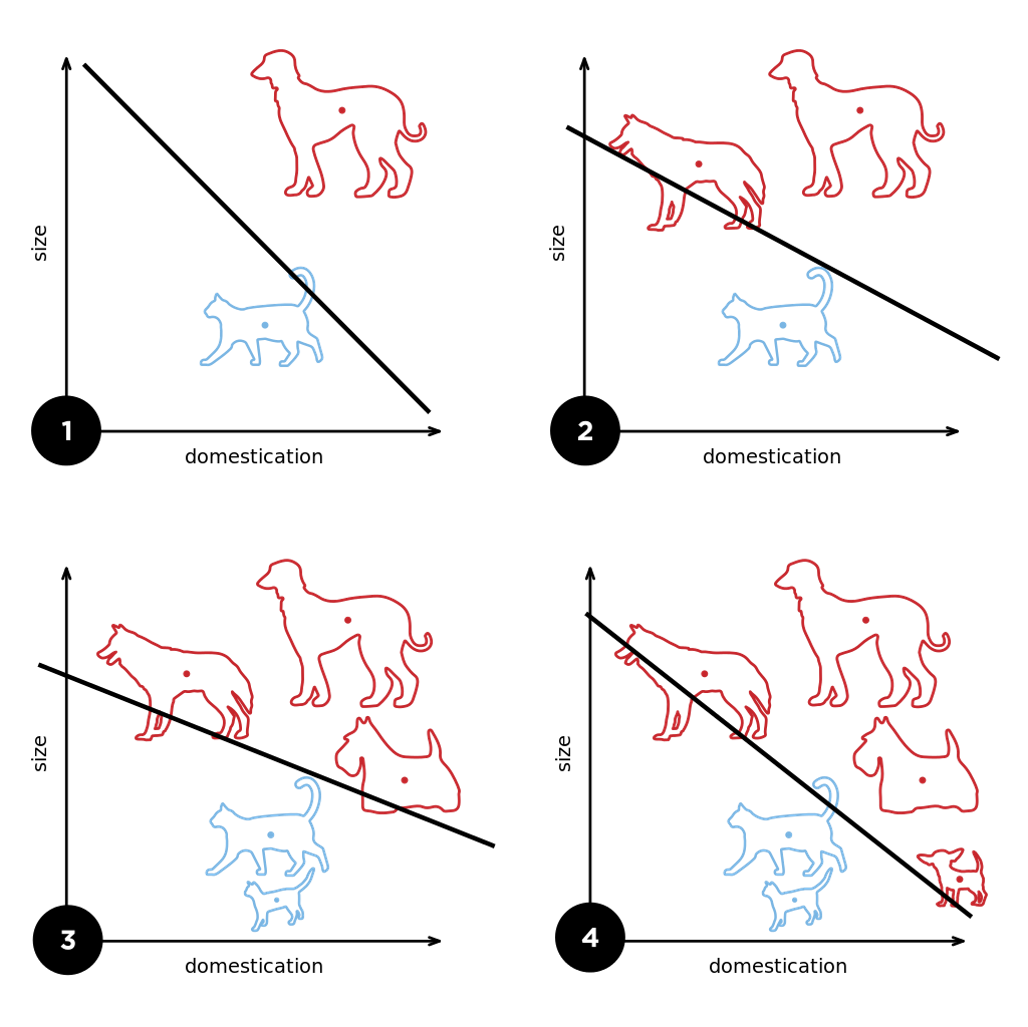
\includegraphics[width=\textwidth]{Perceptron_example}
\caption{A diagram of a perceptron learning to change its linear boundary as more training data is added. In this it is classifying whether an animal is a cat or a dog depending on its size and level of domestication.} 
\label{fig:Perceptron_example} 
\end{subfigure}
~
\begin{subfigure}[t]{0.45\textwidth}
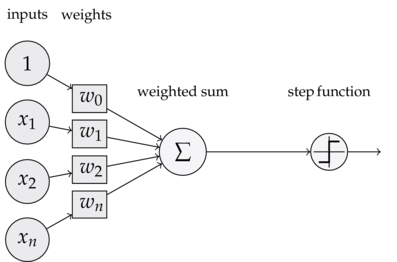
\includegraphics[width=\textwidth]{SingleLayerPerceptron}
\caption{Diagram of a single layer perceptron, as described by Rosenblatt. A feature vector is fed in and a weighted sum is made of the features. A step function is used as an activation to give the binary output of 0 or 1.} 
\label{fig:SingleLayerPerceptron}
\end{subfigure}
\end{figure}

Rosenblatt was highly optimistic about the abilities of the perceptron. However in 1969 Marvin Minsky and Seymour Papert published their book \textit{Perceptrons: an introduction to computational geometry} \cite{Minsky1969Perceptrons:Geometry} in which they proved mathematically that a single layer perceptron could not learn, for example, the XOR logic function. This controversial book signalled the start of the first 'dark age' of machine learning, however it was not to last long.\\
Machine learning research would rise again after the invention of \textit{back propagation}. Back propagation was a new method of learning developed by David Rumelhart, Geoffrey Hinton  and Ronald Williams and published in 1986 \cite{Rumelhart1986LearningErrors}. This paper introduced the idea of a network of 'hidden layers', unlike previous multilayer perceptrons these hidden layers had weights set by a back propagation algorithm, rather than by hand. The back propagation algorithms job was to tune the weights of neurons to reduce the difference between the network output and the desired output. This breakthrough allowed these 'neural networks' to learn non-linear functions, not possible with simple perceptrons. Further papers proved that neural networks could theoretically learn any non-linear function, given enough neurons \cite{Hornik1991ApproximationNetworks}. Early success was had with convolutional neural network used to identify handwritten digits \cite{LeCun1990HandwrittenNetwork}. However funding cuts, expensive systems and a long list of missed goals led an 'AI winter'. With many losing faith in artificial intelligence. This did not stop IBM, who in 1997 beat reigning world chess champion Garry Kasparov with their machine 'Deep Blue', and for the first time showed the capabilities of artificial intelligence. Deep Blue used massively parallel computing to calculate hundreds of millions of positions every second \cite{Campbell2002DeepBlue}. This brute force approach is not the same as other machine learning methods discussed.\\
It was not until the 'big data' revolution of the 21st century that machine learning was truly taken seriously. The mid 2000's saw a series of revolutionary papers that greatly improved the performance of neural networks. Greedy layerwise training was first proposed in 2006 \cite{Bengio2006GreedyNetworks}, as a way to initialise the weights of a neural network before the supervised learning stage. Random initialisation would often lead to poor final solutions. Increasing computing power meant that the power of neural network could finally be realised.

%********************************** %Fourth Section  *************************************

\section{Introduction to Deep Learning} %Section - 1.4
The deep neural network comprises of many hidden layers is the backbone of Deep learning. It has been demonstrated to very capable of image and sound classification, and many other 'big data' problems.

%********************************** %Fifth Section  *************************************

\section{VELO Track Reconstruction} %Section - 1.5
VELO track reconstruction is the name for a series of algorithms that takes hits in the VELO and returns tracks. These tracks are then used for physics analysis. This section will describe the known method for VELO upgrade track reconstruction \cite{Bird:1620453}.

\subsection{Definitions}
Define measurements, clusters, tracks, states etc. \cite{Hernando:1057515}

\subsection{Clustering}
Particles will often deposit energy in more than one pixel in each sensor. A group of pixels belonging to the same hit is known as a cluster. The number of pixels in a cluster is determined by the angle the particle passed through the sensor. A steeper angle will create larger clusters whilst shallower angles will create smaller clusters. Each pixel has a binary readout, meaning a cluster is represented by a small group of 1's in a large array of 0's. The clustering software looks for groups of up to 8 connected hits, these can be connected horizontally, vertically or diagonally.

\subsection{Pattern Recognition}
Clusters are stored with errors $\Delta$x and $\Delta$y. These errors are used for calculating weights for the track fit later in the process, and are approximated by $\Delta x = \Delta y = p/\sqrt{12}$ where $p$ is the size of each pixel.
The method of pattern recognition currently developed works as follows:
\begin{enumerate}
    \item Starting from the most downstream module (module with the largest $z$) pairs of unused clusters in the next upstream module are investigated. These cluster pairs must have track slopes $|dx/dz|<0.4$ and $|dy/dz|<0.4$. The restriction of track slopes is used so that only tracks that lead roughly towards the interaction point are looked at.
    \item Step 1 will produce a number of possible track seeds between every pair of adjacent modules, to determine which seed is correct each track seed is extrapolated to the next upstream module. A small window is drawn around each extrapolated hit in the 3rd module, if there are any clusters inside this window then this cluster will be added to the track.
    \item After this process is complete tracks that contain less than three clusters are rejected. Tracks with exactly three clusters must contain only unused clusters and pass a cut on the track $\chi^2$ from a least-squares fit. Tracks with more contain more than three clusters must at least 50\% unused clusters, if this is true then all clusters are added to the track and tagged as used.
    \item The next stage is to convert each temporary track to a \verb|Track::Velo| object. If the z-position at which the track is closest to the beam line is larger than the maximum z-position of any cluster then the track is labelled as a backward track, otherwise it is labelled as a forward track. The track is then fit using a Kalman filter with scattering. This method if fitting gives better impact parameter resolution than a standard straight line fit. The scattering per layer is approximated by
    $$\sigma_{MS}^{2}=a+b(t_{x}^{2}+t_{y}^{2})$$
    where $t_x$ and $t_y$ are the track slopes and $a$ and $b$ are parameters determined from Monte Carlo simulation.
    \item Finally track states are calculated for each track. A track state is simply an $x,y,z$ coordinate with errors on $x$ and $y$. Track states are calculated for each track at a z-position closest to the beam line and at the end of the VELO (defined as z=770mm).
\end{enumerate}
It is this step I will be trying to improve through the application of machine learning.

\subsection{Parallel method}
The current method is sequential, this means that each layer is looked at individually and tracks built from the outside of the VELO towards the interaction point. Parallel computing can offer large speed ups when a problem involves many small, independent calculations. An attempt to parallelise VELO upgrade pattern recognition has been made and will be described \cite{Ticse:1554078}. However this is not the only example \cite{Abba:1667587}.
\begin{enumerate}
    \item Instead of starting in the outermost module, all modules are looked at simultaneously. Firstly the algorithm finds all pairs of clusters (Tracklets) in given angular range.
    \item Information about each tracklet is stored. These are the slope in x and y $(dx,\ dy)$, and the projection to a plane beyond last velo layer, known as the \textit{e-plane} $(ex,\ ey)$. figure \ref{fig:SIMDVeloPR}
    
    \begin{figure}[h] % h for here in document
    \centering 
    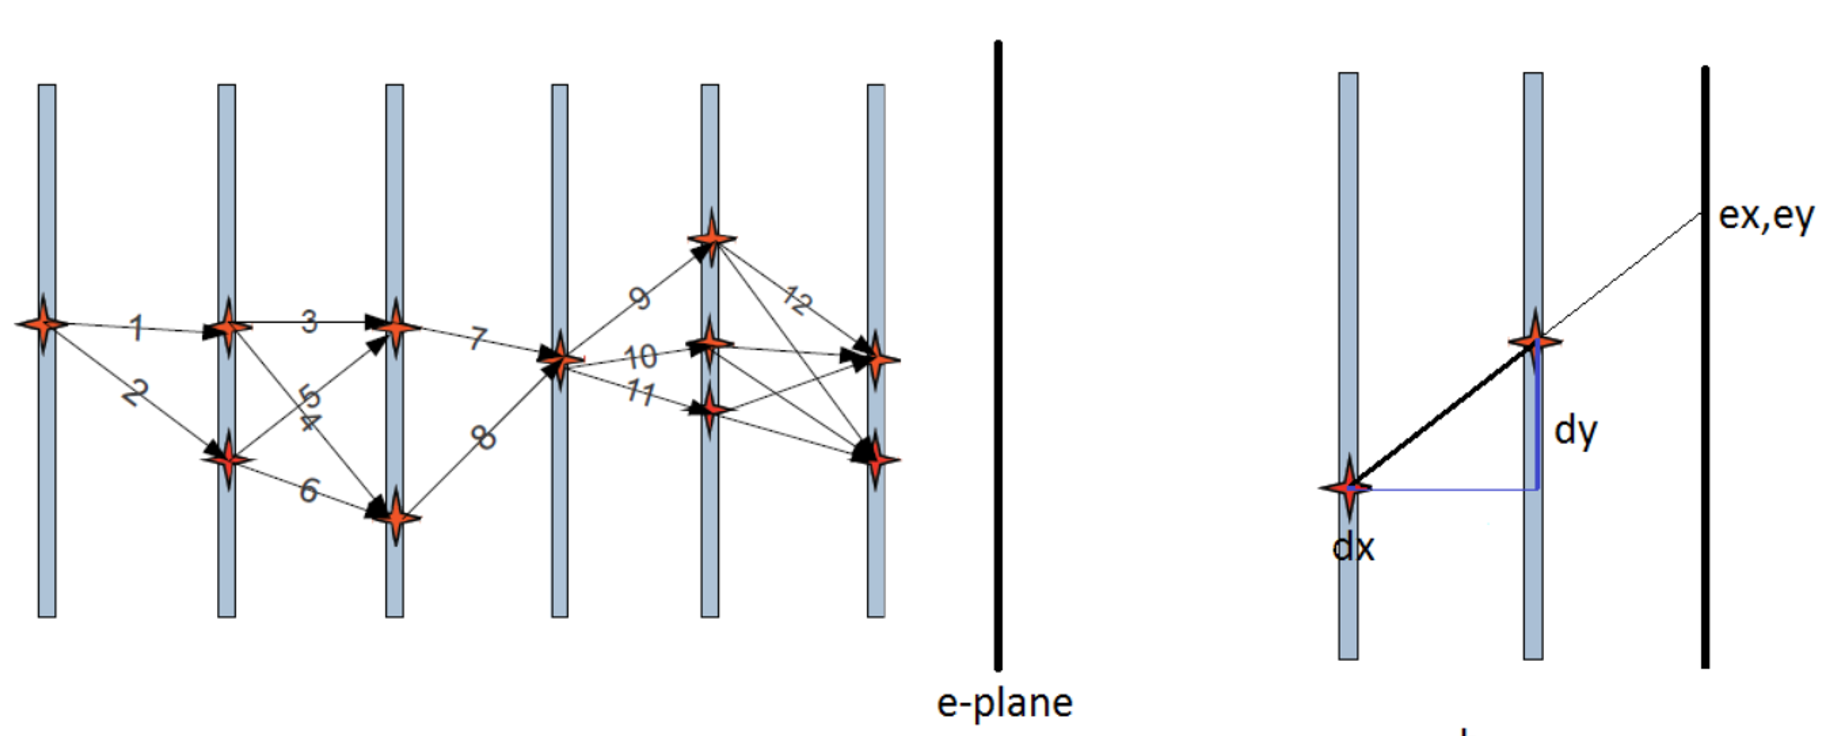
\includegraphics[width=\textwidth]{SIMDVeloPR}
    \caption{Diagram of tracklet formation and definition of parameters.} 
    \label{fig:SIMDVeloPR} 
    \end{figure}

    \item To connect tracklets into tracks calculate the gradient and projection distance for every pair of tracklets. As these distances are independent of each other these can be calculated  quickly in parallel. For each tracklet this will give a list of gradient and projection distances for all other tracklets between different modules. 
    \item Tracklets with similar gradient and projection distance should be part of same track. Groups of tracklets with small gradient and projection distances are probably in the same track. By defining a maximum distance between these distance tracklets can be grouped into tracks.
\end{enumerate}
This method was demonstrated to work well on low density data, with few clusters and tracks. With efficiency and purity up to 88\%. However with high cluster and track densities the efficiency and purity reduced significantly. Down to 55\% efficiency and 3\% purity.\\
Efficiency is defined as the number of correctly reconstructed tracks divided by the number of tracks. And purity is defined as ...\\
This method is not fully developed and has many areas in need of improvement. However it is still an interesting look into speeding up the pattern recognition system.


\subsection{Efficiency}
Monte Carlo simulation truth can be used to calculate the efficiency of this method. The efficiency is calculated by comparing the number of correctly reconstructed tracks to the number of reconstructible tracks from the MC. The following definitions are used by LHCb:

\begin{itemize}
    \item A track is reconstructible as a VELO track if there are clusters associated to it on three or more modules
    \item A track is reconstructible as a “long track” if it is reconstructible as a VELO track and, in addition, has at least one x and one “stereo” hit in each of the three downstream track seeding stations.
    \item A particle is considered reconstructed if at least 70\% of the measurements on a track are associated to this particle.
    \item A ghost track or fake track is a track which cannot be associated to any simulated particle.  If more than one reconstructed track is associated to a particle the extra tracks are counted as clone tracks.
    \item $\epsilon_{rec}=\frac{N_{correctly\ reconstructed}}{N_{reconstructible}}$
\end{itemize}
The method described above can achieve very high efficiency's of >99\%, more than that of the current VELO \cite{Collaboration:1624070}. However it is not optimised for speed.


%*******************************************************************************
%****************************** Second Chapter *********************************
%*******************************************************************************

\chapter{First Steps}

\ifpdf
    \graphicspath{{Chapter2/Figs/Raster/}{Chapter2/Figs/PDF/}{Chapter2/Figs/}}
\else
    \graphicspath{{Chapter2/Figs/Vector/}{Chapter2/Figs/}}
\fi


\section[Short title]{Reasonably long section title}

\chapter{Results}

% **************************** Define Graphics Path **************************

\graphicspath{{Figs/}}

%********************************** %First Section  **************************************

\section{Pixels} %Section - 1.1 
Before any data could be fed into a cnn the data had to be formatted correctly. To simulate a grid of pixels from the xyz coordinate data the points were binned, with the number of bins representing the number of pixels in the x and y directions. The future VELO sensors are square 256x256 arrays of pixels, arranged 3 in a row, and 2 of these sensor triplets arranged in an L shape. [Insert diagram of VELO module]. To give relative realism to the binning process 1024 bins were used, giving an image with 1048576 total pixels. [Insert image of input layer]. However this method is very memory intensive and would crash when running on my laptop. Therefore the decision was made to down sample the image to 128x128 pixels, 16384 total pixels. This would allow it to run while not impacting on the images formed, by this I mean down sampling did not lead to a situation where 2 hits ended up in the same pixel. Various combinations of convolutional and fully connected layers were tried and tested but with few satisfactory results. There was promise when the network first started ‘learning’, ie the loss reduced over time. However on closer inspection it was found that the network was doing this by simply setting all pixel values to 0. An attempt to improve performance was made by designating which parts of the xy plane expected hits and which areas were not active pixel regions. [Insert image of new input layer]. This had little effect on performance.

\subsection{Results}

\subsection{Discussion}

%********************************** %Second Section  **************************************

\section{Points} %Section - 1.2
After having very little success with this ‘pixel’ method I changed direction. Instead of taking the xyz coordinates of each hit and turning it into an image, the raw xyz coordinates were used directly. This will most likely be the method of the eventual solution. The method of formatting the data was as follows. Take the xyz coordinates for 2 layer of the detector, since particle id is known and given, remove any hits that do not appear in both layers, this is helpful as it means we know which x and y points in 1 layer correspond to the xy points in the next layer. Create 1d arrays for the x and y coordinates of each hit for every event in each mdbatch data file, each array has the format (x0, y0, x1, y1, …, xn, yn). The hits from the first layer are the data, the hits from the second layer are the labels. Each array was split to create 6 final arrays. Training data, testing data, validation data, validation labels, testing data, testing labels. These were saved as datasets into an h5py file for fast reading and writing of data.
The configuration of the neural network was different for this ‘points’ method. It was first thought that a problem with this method was that each event has a different number of points, and neural networks need a consistent size input and output. The solution to this is to feed in one xy point at a time. So the network had input and output sizes of 2. This means 1 xy pair is trained on each time. The network had one fully connected hidden layer of size 1024.
The ‘points’ method has had promising results. For outer layers of the VELO it is very good at predicting hits in the next layer. But is less accurate for layers closer to the collision point. [Insert images of outputs].

\begin{figure}[h] % h for here in document
\centering
\begin{subfigure}[t]{0.45\textwidth}
\centering
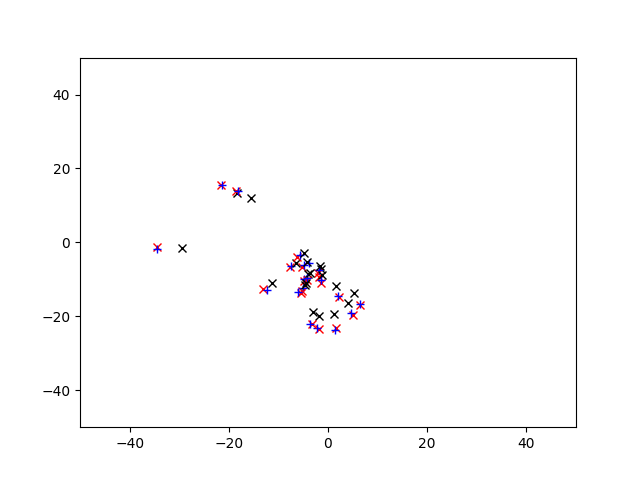
\includegraphics[width=\textwidth]{Figs/layers-136-161}
\caption{} 
\label{fig:2a} 
\end{subfigure}
~
\begin{subfigure}[t]{0.45\textwidth}
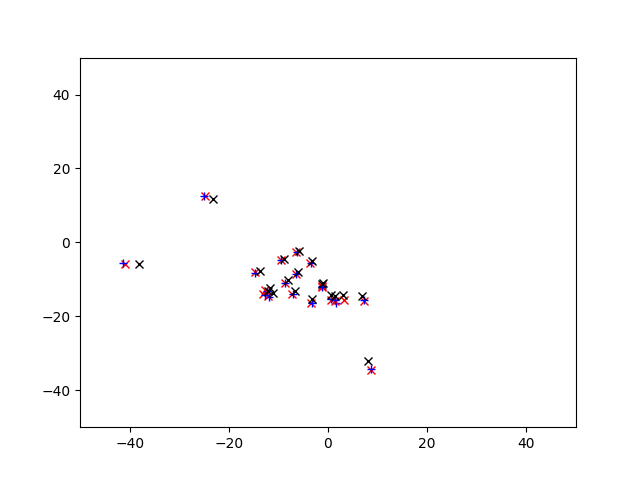
\includegraphics[width=\textwidth]{Figs/layers-686-736}
\caption{} 
\label{fig:2b}
\end{subfigure}
\end{figure}


\subsection{Results}

\subsection{Discussion}

%********************************** %Second Section  **************************************

\section{Closest numbers and points} %Section - 1.3
I was tasked with creating a neural net that could use a set of 8 random numbers as an input and output the pair that have the smallest difference. This would then lead on to finding the closest pair of 2-vectors from a random set. The long term aim of this is to develop a system that can connect 2D points into tracks.
Most effort was involved in creating data files in the correct format. Supervised learning requires labels that the neural network output can be tested against. A logical label would have the format of an array of zeros for each input number or vector, with a 1 value for the two points that are the closest together. With this problem solved it is a relatively simple job to setup a neural network model using Keras as a front end to Tensorflow. Initial accuracy's of ~96\% for 1 million samples of random points were encouraging.\\

The accuracy of this method was tested further to fully understand the neural network output.

\begin{figure}[h] % h for here in document
\centering
\begin{subfigure}[t]{0.45\textwidth}
\centering
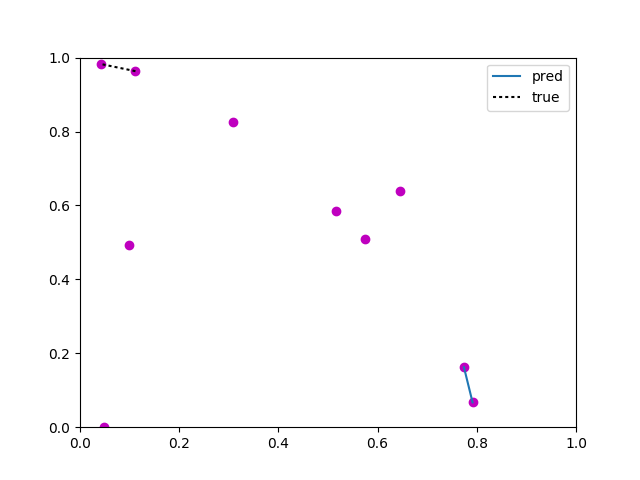
\includegraphics[width=\textwidth]{Figs/closest_dist_fail2.png}
\caption{An example of a failure case} 
\label{fig:3a} 
\end{subfigure}
~
\begin{subfigure}[t]{0.45\textwidth}
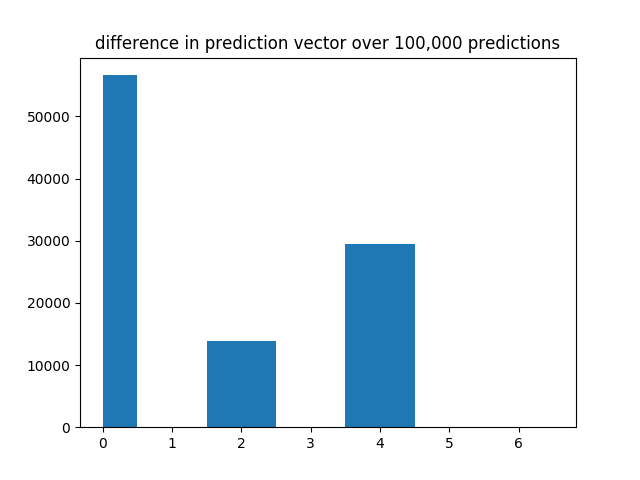
\includegraphics[width=\textwidth]{Figs/pred_dif_hist.png}
\caption{A histogram representing the output of the neural network} 
\label{fig:3b}
\end{subfigure}
\end{figure}

The output of the neural network was a vector of zeros with length 10. Two 1's in this vector represent the two points to be connected. If there was a 1 at position 2 and position 4 then points 2 and 4 were deemed the closest pair.

\[
\begin{pmatrix}
0 & 0 & 1 & 0 & 1 & 0 & 0 & 0 & 0 & 0
\end{pmatrix}
\]

To investigate the output of the network the difference between the predicted and true vectors was calculated. This was done by taking the absolute of element wise subtraction. Therefore if the predicted vector was the same as the true vector then the difference would be 0. If one point was incorrectly classified then the difference would be 2. And finally if both points were incorrectly classified then the difference would be 4. The histogram in Figure... shows this over all 100000 testing samples. The majority are correctly classified (57\%), some have one incorrect classification (14\%) and some have two incorrect classifications (29\%). These numbers are nowhere near the 96\% claimed accuracy, this does not mean however, that the network is bad at finding pairs of closest points. Failure cases were investigated to understand. figure a shows one failure case. The nerual network has found a pair of points with a distance apart very close to the true closest pair. For the intended application in particle physics this is a very satisfactory result.


\subsection{Results}

\subsection{Discussion}

%********************************** %Second Section  **************************************

\section{Joining the dots} %Section - 1.4 
After initial success of finding the two closest points I moved onto connecting more points together to 'join the dots'. This was defined as finding the two closest points, then from one of these points finding the next closest. This was achieved by...\\
Finding the two closest points is an established problem which can be solved quickly.\\
The next step was to use the neural network for the entire process, finding the two closest points and then joining the dots. It was important to find the correct way to represent the connections between points. Many different ways were tried. Firstly using the adjacency matrix of the points, then using the indices of the points was tried, also simply using the network to give back the coordinates in the connected order.\\
Only one method worked well. that was to train the neural network to output the undirected adjacency matrix of the points. An adjacency matrix is an n x n matrix, for n points, which shows which points are connected to each other. There are 0's where there is no connection, and 1's where there is a connection. So, for example, if points 2 and 3 are connected, there will be a 1 in the 2nd row and 3rd column of the adjacency matrix. However there will also be a 1 in the 3rd row and 2nd column, as the direction of the connection is not important. \\

\[
\begin{pmatrix}
0 & 0 & 0 & 0 \\
0 & 0 & 0 & 0 \\
0 & 0 & 0 & 1 \\
0 & 0 & 1 & 0
\end{pmatrix}
\]

The neural network was fed sets of 10 random 2d points with x and y ranging between 0 and 1. The adjacency matrix for each set of 10 points was calculated. To start 1 million sets of random numbers were used, 80\% for training, 10\% for validation and 10\% for testing. After inital testing gave encouraging results 5 million sets of random numbers and corresponding adjacency matrices were generated.\\

Here I will include results.

\section{Receiver Operating Codes}
Results must have an error metric so that they can be compared. The language of receiver operating codes fits well in this context. The true connections between points are calculated so that the neural networks can be trained. Therefore the neural network output can be correct or incorrect in these ways:
\begin{itemize}
    \item True Positive (TP) - A connection was made when it should have been.
    \item True Negative (TN) - A connection was not made when it should not have been.
    \item False Positive (FP) - A connection was made when it should not have been.
    \item False Negative (FN) - A connection was not made when it should have been.
\end{itemize}
To understand the numbers of these outcomes the Sensitivity and Specificity are calculated.
\[ Sensitivity = \frac{TP}{TP + FN} \]
\[ Specificity = \frac{TN}{TN + FP} \]

Both these metrics must be high in order to have satisfactory results. If the sensitivity is high but the specificity is low then this indicates the neural network is connecting all points together, this will make sure all correct connections are made. If the specificity is high but the sensitivity is low then the network will not connect any points together. Therefore a balance is needed for good performance\\
A ROC curve is a plot of Sensitivity against 1-Specificity over some parameter. In my case the parameter was the threshold of the neural network output. Thanks to the last layer having a Sigmoid activation function each element of the output was a number between 0 and 1. The adjacency matrix must only contain 0's and 1's so a threshold was used, any output element below the threshold was set to 0, and any element above the threshold was set to 1. Plotting the ROC curve allows for tuning of the threshold to an optimum. The further to the top and left the ROC curve goes indicates better performance.
\textbf{}

\subsection{Results}

\subsection{Discussion}
%\include{Chapter4/chapter4}
%\include{Chapter5/chapter5}
%\include{Chapter6/chapter6}
%\include{Chapter7/chapter7}



% ********************************** Back Matter *******************************
% Backmatter should be commented out, if you are using appendices after References
%\backmatter

% ********************************** Bibliography ******************************
\begin{spacing}{0.9}

% To use the conventional natbib style referencing
% Bibliography style previews: http://nodonn.tipido.net/bibstyle.php
% Reference styles: http://sites.stat.psu.edu/~surajit/present/bib.htm

%\bibliographystyle{apalike}
\bibliographystyle{plainnat} % use this to have URLs listed in References
\cleardoublepage
\bibliography{References/references} % Path to your References.bib file


% If you would like to use BibLaTeX for your references, pass `custombib' as
% an option in the document class. The location of 'reference.bib' should be
% specified in the preamble.tex file in the custombib section.
% Comment out the lines related to natbib above and uncomment the following line.

%\printbibliography[heading=bibintoc, title={References}]


\end{spacing}

% ********************************** Appendices ********************************

%\begin{appendices} % Using appendices environment for more functunality

%% ******************************* Thesis Appendix A ********************************
\chapter{How to install \LaTeX} 

\section*{Windows OS}

\subsection*{TeXLive package - full version}
\begin{enumerate}
\item	Download the TeXLive ISO (2.2GB) from\\
\href{https://www.tug.org/texlive/}{https://www.tug.org/texlive/}
\item	Download WinCDEmu (if you don't have a virtual drive) from \\
\href{http://wincdemu.sysprogs.org/download/}{http://wincdemu.sysprogs.org/download/}
\item	To install Windows CD Emulator follow the instructions at\\
\href{http://wincdemu.sysprogs.org/tutorials/install/}{http://wincdemu.sysprogs.org/tutorials/install/}
\item	Right click the iso and mount it using the WinCDEmu as shown in \\
\href{http://wincdemu.sysprogs.org/tutorials/mount/}{http://wincdemu.sysprogs.org/tutorials/mount/}
\item	Open your virtual drive and run setup.pl
\end{enumerate}

or

\subsection*{Basic MikTeX - TeX distribution}
\begin{enumerate}
\item	Download Basic-MiK\TeX (32bit or 64bit) from\\
\href{http://miktex.org/download}{http://miktex.org/download}
\item	Run the installer 
\item	To add a new package go to Start >> All Programs >> MikTex >> Maintenance (Admin) and choose Package Manager
\item	Select or search for packages to install
\end{enumerate}

\subsection*{TexStudio - Tex Editor}
\begin{enumerate}
\item	Download TexStudio from\\
\href{http://texstudio.sourceforge.net/\#downloads}{http://texstudio.sourceforge.net/\#downloads} 
\item	Run the installer
\end{enumerate}

\section*{Mac OS X}
\subsection*{MacTeX - TeX distribution}
\begin{enumerate}
\item	Download the file from\\
\href{https://www.tug.org/mactex/}{https://www.tug.org/mactex/}
\item	Extract and double click to run the installer. It does the entire configuration, sit back and relax.
\end{enumerate}

\subsection*{TexStudio - Tex Editor}
\begin{enumerate}
\item	Download TexStudio from\\
\href{http://texstudio.sourceforge.net/\#downloads}{http://texstudio.sourceforge.net/\#downloads} 
\item	Extract and Start
\end{enumerate}


\section*{Unix/Linux}
\subsection*{TeXLive - TeX distribution}
\subsubsection*{Getting the distribution:}
\begin{enumerate}
\item	TexLive can be downloaded from\\
\href{http://www.tug.org/texlive/acquire-netinstall.html}{http://www.tug.org/texlive/acquire-netinstall.html}.
\item	TexLive is provided by most operating system you can use (rpm,apt-get or yum) to get TexLive distributions
\end{enumerate}

\subsubsection*{Installation}
\begin{enumerate}
\item	Mount the ISO file in the mnt directory
\begin{verbatim}
mount -t iso9660 -o ro,loop,noauto /your/texlive####.iso /mnt
\end{verbatim}

\item	Install wget on your OS (use rpm, apt-get or yum install)
\item	Run the installer script install-tl.
\begin{verbatim}
	cd /your/download/directory
	./install-tl
\end{verbatim}
\item	Enter command `i' for installation

\item	Post-Installation configuration:\\
\href{http://www.tug.org/texlive/doc/texlive-en/texlive-en.html\#x1-320003.4.1}{http://www.tug.org/texlive/doc/texlive-en/texlive-en.html\#x1-320003.4.1} 
\item	Set the path for the directory of TexLive binaries in your .bashrc file
\end{enumerate}

\subsubsection*{For 32Bit OS}
For Bourne-compatible shells such as bash, and using Intel x86 GNU/Linux and a default directory setup as an example, the file to edit might be \begin{verbatim}
edit $~/.bashrc file and add following lines
PATH=/usr/local/texlive/2011/bin/i386-linux:$PATH; 
export PATH 
MANPATH=/usr/local/texlive/2011/texmf/doc/man:$MANPATH;
export MANPATH 
INFOPATH=/usr/local/texlive/2011/texmf/doc/info:$INFOPATH;
export INFOPATH
\end{verbatim}
\subsubsection*{For 64Bit}
\begin{verbatim}
edit $~/.bashrc file and add following lines
PATH=/usr/local/texlive/2011/bin/x86_64-linux:$PATH;
export PATH 
MANPATH=/usr/local/texlive/2011/texmf/doc/man:$MANPATH;
export MANPATH 
INFOPATH=/usr/local/texlive/2011/texmf/doc/info:$INFOPATH;
export INFOPATH

\end{verbatim}



%\subsection{Installing directly using Linux packages} 
\subsubsection*{Fedora/RedHat/CENTOS:}
\begin{verbatim} 
sudo yum install texlive 
sudo yum install psutils 
\end{verbatim}


\subsubsection*{SUSE:}
\begin{verbatim}
sudo zypper install texlive
\end{verbatim}


\subsubsection*{Debian/Ubuntu:}
\begin{verbatim} 
sudo apt-get install texlive texlive-latex-extra 
sudo apt-get install psutils
\end{verbatim}

%% ******************************* Thesis Appendix B ********************************

\chapter{Installing the CUED Class file}

\LaTeX.cls files can be accessed system-wide when they are placed in the
<texmf>/tex/latex directory, where <texmf> is the root directory of the user’s \TeX installation. On systems that have a local texmf tree (<texmflocal>), which
may be named ``texmf-local'' or ``localtexmf'', it may be advisable to install packages in <texmflocal>, rather than <texmf> as the contents of the former, unlike that of the latter, are preserved after the \LaTeX system is reinstalled and/or upgraded.

It is recommended that the user create a subdirectory <texmf>/tex/latex/CUED for all CUED related \LaTeX class and package files. On some \LaTeX systems, the directory look-up tables will need to be refreshed after making additions or deletions to the system files. For \TeX Live systems this is accomplished via executing ``texhash'' as root. MIK\TeX users can run ``initexmf -u'' to accomplish the same thing.

Users not willing or able to install the files system-wide can install them in their personal directories, but will then have to provide the path (full or relative) in addition to the filename when referring to them in \LaTeX.



%\end{appendices}

% *************************************** Index ********************************
\printthesisindex % If index is present

\end{document}
